%%%%%%%%%%%%%%%%%%%%%%%%%%%%%%%%%%%%%%%%%%%%%%%%%%%%%%%
% A template for Wiley article submissions.
% Developed by Overleaf.
%
% Please note that whilst this template provides a
% preview of the typeset manuscript for submission, it
% will not necessarily be the final publication layout.
%
% Usage notes:
% The "blind" option will make anonymous all author, affiliation, correspondence and funding information.
% Use "num-refs" option for numerical citation and references style.
% Use "alpha-refs" option for author-year citation and references style.

\documentclass[num-refs]{wiley-article}
% \documentclass[alpha-refs]{wiley-article}

% Add additional packages here if required
\usepackage{siunitx}
\usepackage{amsmath}
\usepackage{bm}
\usepackage{graphicx}
\usepackage[inline]{enumitem}
\usepackage{caption}
\usepackage{subcaption}
\usepackage{float}
\usepackage{longtable}
\usepackage{tabularx}
\usepackage{setspace}
\usepackage{amssymb}
\usepackage[colorlinks=true]{hyperref}
% \usepackage{endfloat}

% Image path declaration
% \graphicspath{{./figure/bw/}} % Black and white figures
\graphicspath{{./figure/color/}} % Color figures

% hyperref setup
\colorlet{myblue}{blue!50!black}
\colorlet{mybrown}{brown!50!black}
\colorlet{mygreen}{green!50!black}

\hypersetup{
  linkcolor = mybrown,
  citecolor = myblue,
  urlcolor = mygreen,
}

% Initialize theorems and propositions
%\newtheorem{theorem}{Theorem}
%\newtheorem{principle}{Principle}
%\newtheorem{proposition}{Proposition} \theoremstyle{remark}
%\newtheorem{example}{Example}

% Update article type if known
\papertype{Original Article}
% Include section in journal if known, otherwise delete
\paperfield{Journal Section}

\title{Model and estimators for partial least squares regression. \\
  Running title: Model and estimators for PLS.}

% List abbreviations here, if any. Please note that it is preferred that abbreviations be defined at the first instance they appear in the text, rather than creating an abbreviations list.

% \abbrevs{PLS, a black cat; DEF, doesn't ever fret; GHI, goes home immediately.}

% Include full author names and degrees, when required by the journal.
% Use the \authfn to add symbols for additional footnotes and present addresses, if any. Usually start with 1 for notes about author contributions; then continuing with 2 etc if any author has a different present address.

% \author[1\authfn{1}]{Inge Svein Helland}
\author[1]{Inge Svein Helland}
\author[2]{Solve S\ae b\o}
\author[2]{Trygve Alm\o y}
\author[2]{Raju Rimal}

% \contrib[\authfn{1}]{corresponding author}

% Include full affiliation details for all authors
\affil[1]{University of Oslo}
\affil[2]{Norwegian University of Life Sciences}

\corraddress{Department of Mathematics, \href{http://uio.no}{University of Oslo}, P.O. Box 1053, NO-0316 Oslo, Norway}
\corremail{ingeh@math.uio.no}

% \presentadd[\authfn{2}]{Department of Mathematics, \href{http://uio.no}{University of Oslo}, P.O. Box 1053, NO-0316 Oslo, Norway}

\fundinginfo{Funding Information}

% Include the name of the author that should appear in the running header
\runningauthor{Inge Svein Helland et al.}

\begin{document}

\maketitle

\begin{abstract}
Partial least squares regression has been a very popular method for prediction. The method can in a natural way be connected to a statistical model which now has been extended and further developed in terms of an envelope model. Concentrating on the univariate case, several estimators of the regression vector in this model are defined, including the ordinary PLS estimator, the maximum likelihood envelope estimator and a recently proposed Bayes PLS estimator. These are compared with respect to prediction error by systematic simulations. The simulations indicate that Bayes PLS performs well compared to the other methods.

% Please include a maximum of seven keywords
\keywords{Bayes PLS estimator, envelope model, maximum likelihood envelope estimator, partial least squares, partial least squares model, simulation}

\end{abstract}

\section{Introduction}

Supervised learning from multivariate data is a central problem area in applied statistics and also in chemometrics. Specifically, let our task be to predict a single variable $y$ from a $p$-dimensional variable $\bm{x}$, having data on $n$ units. From a statistical point of view a large number of learning methods are discussed in \citet{hastie2009elements}, mainly under the ordinary multiple regression model. In chemometrics, partial least squares (PLS) regression is the dominating method.

Partial least squares regression has had a vigorous devolopment in the
chemometric literature since it was proposed by Herman and Svante Wold and by
Harald Martens \citep{wold1983collinearity, martens1989multivariate}. The method
has been extended in several directions and its applications have been expanded
to an increasing number of fields, for instance genomic data
\citep{boulesteix2007partial}. Both these issues have been discussed in detail
in a recent paper by \citeauthor{mehmood2016diversity} \citet{mehmood2016diversity}, where a wealth of further references may be found.

In the beginning the PLS method was to some extent neglected or turned down by statisticians (an exception among others was \citealp{frank1993statistical}), but it is now included as a tool among other biased regression methods by applied statisticians. For a general discussion paper with contributions both from mathematical statisticians and chemometricians, see \citet{sundberg1999multivariate}.

Indeed there was a difference in culture between chemometricians and statisticians then, and this difference still exists to a large extent. A statement by Munck et al.  \citet{munck2010physiochemical} illustrates this, as seen from one side: 'If chemometrics in its historical development had been limited to follow current scientific (and statistical) theories there would have been minimal progress in its wide applications today.'

Recently, the difference in culture was discussed in some detail by Harald Martens \citet{martens2015bigdata}. On the one hand, Martens makes the point that the field of Chemometrics has a lot to learn from other disciplines -- mathematics, statistics and computer science. Among other things, he says that it will not be enough to have efficient `black box' algorithms. On the other hand he accuses statisticians in general for a predilection for `macho mathematics', concluding in part that Chemometrics need more statistics, but not more statisticians. In other parts of the paper he talks about bridging the gap between the two disciplines, an effort that we whole-heartedly support.

This difference in culture may in part be related to the concepts of creativity and rigor, qualities which to some extent may be called complementary. One could say that one culture puts more emphasis on creativity, the other on rigor. Of course, this is a huge simplification. First, there is a lot of creativity among statisticians, also mathematical statisticians. Secondly, one should emphasize that precise thinking also should influence practice. A case of point is the following:  Chung and Keles \citet{chung2010sparse} recently proved that the PLS regression vector is inconsistent when $p/n\rightarrow k>0$ under a wide set of conditions. This result is probably not too well known among chemometricians; some may have a tendency to put much confidence in PLS regression when $p\sim n$ or $p>n$. It is to be emphasized that the inconsistency result in \citet{chung2010sparse} is only concerned with estimation of the regression vector. The mathematical properties of PLS as a \emph{prediction} method when $p>n$ are largely unknown, from a statistical point of view. There is much positive empirical evidence among applied researchers on these properties, but statisticians have only started to attack this problem, since it from an analytic point of view is very difficult. In particular, see the very recent paper by Cook and Forzany \citet{cook2017pls} where asymptotic expansions allowing both $n$ and $p$ to be large are developed for PLS prediction with one component.

It is true that chemometricians have had a leading edge in the development of PLS and of certain multivariate methods, in particular with respect to visualization etc., and they still are ahead of statisticians in this sense.

Accepting this, an important general question is what mathematical statisticians can contribute with in this development. A vital aspect in the history of statistics is the interplay between model and estimators. Once a model is formulated, one can in principle think of several estimators in this model. A statistician will talk about a `hard' model in terms of probability distributions -- at least in terms of a model equation and a statement of correlation between terms in this model. This is a concept that has had and has a great success in a number of disciplines, and is at the very core of statistics as a science. Our goal in the present paper is to show that this concept can be applied -- and is useful -- also in connection to PLS. Specifically our purposes are to

\begin{itemize}[label={--}]
\item stress that PLS as an algorithm can be connected to a unique statistical model (known since 1990);
\item formulate 5 different ways to present this model (known in the statistical literature since 2013);
\item argue that the simplest way to present the model is through the concept of relevant components - a reduction of the random $x$ regression model;
\item review briefly some statistical investigations related to PLS;
\item ask if the PLS algorithm may be improved by modifying the weights;
\item argue that once the model is presented, the comparison of different estimators in the model is relevant;
\item present a systematic tool ({\tt simrel}) for comparing estimators in the model with relevant components;
\item present the maximum likelihood estimator in the model;
\item present a Bayes estimator connected to the model;
\item compare the PLS algorithm, the maximum likelihood estimator and the Bayes estimator and the Bayes estimator in a systematic simulation study, mainly with near collinear data.
\end{itemize}


Thus in the PLS model one can certainly discuss other estimators than the usual PLS regression estimator, which can be seen as originating by replacing population (co-)variances in the model by sample (co-)variances. Two examples are the maximum likelihood estimator of \citet{cook2013envelopes}, see also \citet{cook2015envlp}, \citet{cook2016note} and \citet{cook2016algorithms}; and the Bayesian estimator of \citet{helland2012near}. By simulation, both these estimators have performed well compared to PLS regression under certain conditions, but they have their disadvantages. The maximum likelihood estimator can not be used in the case when the data matrix has rank less than $p$, and the Bayesian estimator requires heavy computations, in particular when $p$ is large.

To compare estimators we make vital use of the recently developed simulation package {\tt simrel}; see \citet{saebo2015simrel}. It is very important to have such a tool in an area where it is difficult to obtain results by purely analytical means.

We emphasize that this paper is based upon reduction of the \emph{random} $\bm{x}$ regression model. When considering latent variables from PLS, and when considering near collinearity in the observed $\bm{x}$-variables, it is natural to treat these $\bm{x}$-variables as random. It is our philosophy that this is also the best way to look upon model reduction. On the other hand, in the context of prediction, one could argue that one should condition upon the $\bm{x}$-variables and consider them as fixed. A prominent paper on PLS regression, taking fixed $\bm{x}$-variables in the basic model, is \citet{kramer2012degrees}, where further references can be found.

In recent years there has been a rapidly growing statistical literature on the envelope model - a model generalizing the PLS model. In addition to the maximum likelihood estimation paper mentioned above, the most important papers seem to be \citet{cook2015simultaneous}, where simultaneous reduction in the $\bm{x}$-space and $\bm{y}$-space is proposed, and \citet{cook2015foundations}, where extensions to other regression methods than linear regression are discussed. More references can be found in these papers.

Model reduction in regression models is discussed in general from the point of view of rotations in the $x$-space in \citet{helland2001reduction}.

The plan or this paper is as follows: In Section 2 we formulate the model in 5 different ways which can be shown to be equivalent. In Section 3 we discuss briefly statistical contributions to the study of PLS regression and the PLS model. In Section 4 we define 4 different estimators in the model. In Section 5 we ask the question if the ordinary PLS estimator with $m$ components can be improved by forcing the weight vector at step $m+1$ to vanish; the answer turns out to be negative. Then in Section 6 we define the Bayes PLS estimator of \citet{helland2012near}. In Section 7 we describe the simulations done for comparison of estimators with respect to prediction error, and in Section 8 we give the results of the simulations. Finally, Section 9 is a discussion section.

\section{The model; several formulations}

Take as a point of departure the linear model
\begin{equation}
  \label{model}
  y=\mu_{y}+\bm{\beta}'(\bm{x}-\bm{\mu}_{x})+\epsilon,
\end{equation}
where $\bm{\beta}$ and $\bm{x}$ are $p$-dimensional, and where the random predictor $\bm{x}$ has mean $\bm{\mu}_{x}$ and covariance matrix $\bm{\Sigma}_{xx}$, for simplicity assumed nonsingular here. (This can be relaxed to assuming $\bm{\beta}\in\mathrm{span}(\bm{\Sigma}_{xx})$ in the case where this matrix is singular; see \citet{cook2013envelopes}, and also C below.) Independently, $\epsilon$ is distributed with mean $0$ and variance $\sigma^2$. When doing prediction from this model for near collinear data, a model reduction may be called for. Throughout this paper, a definite $m$-dimensional model reduction, which may be formalized in several equivalent ways, will be used. When this model holds, we say that we have an envelope model or a PLS model of dimension $m$, or that there are $m$ relevant components for prediction in the model. \smallskip

\begin{enumerate}[label=\Alph*.]

\item Given a subspace $\cal{S}$ of $R^p$, let $\bm{P}_{\cal{S}}$ be the projection upon $\cal{S}$, and let $\bm{Q}_{\cal{S}}$ be the projection orthogonal to $\cal{S}$. For simplicity discuss the case where $\bm{\mu}_x =\bm{0}$. Let now $\cal{S}$ be the smallest space such that (i) $\bm{Q}_{\cal{S}}\bm{x}$ is uncorrelated with $\bm{P}_{\cal{S}}\bm{x}$; (ii) $y$ is uncorrelated with $\bm{Q}_{\cal{S}}\bm{x}$ given $\bm{P}_{\cal{S}}\bm{x}$. In this case we may say that $\bm{Q}_{\cal{S}}\bm{x}$ contains no linear information about $y$, neither directly nor through $\bm{P}_{\cal{S}}\bm{x}$. Consider a reduction of the data to $\bm{P}_{\cal{S}}\bm{x}$.
  \smallskip

\item  Here is an algebraic characterization which turns out to be equivalent. For a matrix $\bm{M}$ define $\bm{M}\cal{S}$ as the space of vectors $\bm{Mz}$ as $\bm{z}$ runs through $\cal{S}$, and let $\cal{S}^\perp$ be
  the space perpendicular to $\cal{S}$. Let now $\cal{S}$ be the smallest space in $R^p$ such that (i) both $\bm{\Sigma}_{xx}\cal{S}\subseteq\cal{S}$ and
  $\bm{\Sigma}_{xx}\cal{S}^\perp\subseteq\cal{S}^\perp$; (ii) $\mathrm{span}(\bm{\beta})\subseteq\cal{S}$. In this case we say that $\cal{S}$
  is the envelope of $\mathrm{span}(\bm{\beta})$. It can be shown \citep{cook2010envelope} that the envelope always exists as the smallest space with the stated properties.
  \smallskip

\item The regression vector $\bm{\beta}$ can always be expanded in terms of the eigenvectors $\bm{d}_{i}$ of $\bm{\Sigma}_{xx}$:
  \begin{equation}
    \bm{\beta}=\sum_{i=1}^p \gamma_{i}\bm{d}_{i}.
    \label{beta}
  \end{equation}

  Assume that this sum can be reduced to exactly $m$ non-zero terms:
  $\bm{\beta}=\sum_{i=1}^m \gamma_{i}\bm{d}_{i}$, where the $\bm{d}_i$ correspond to different eigenvalues of $\bm{\Sigma}_{xx}$. We then say that there are $m$ relevant components for prediction in the model. This reduction can be imagined to take place by two mechanisms: 1) Some of the $\gamma_i$'s are really zero. 2) There are coinciding eigenvalues in $\bm{\Sigma}_{xx}$. Then one can rotate such that it is enough with one eigenvector for each eigenspace in the sum. In this approach it is important that we only know that there are $m$ non-zero terms in the sum, not which  terms that are non-zero. For a closer discussion of this, see \citet{naes1993relevant} and \citet{helland1994comparison}.
  \smallskip

\item Consider the  population version of the well known PLS algorithm: Take
  $\bm{e}_{0}=\bm{x}-\bm{\mu}_{x}$, $f_{0}=y-\mu_{y}$, and for $a=1,2,...,m$ compute successively:
  \begin{equation} \label{wt}\bm{w}_{a}=\mathrm{cov}(\bm{e}_{a-1}, f_{a-1}),\ \ \
    t_{a}=\bm{w}_{a}'\bm{e}_{a-1},\end{equation}
  \begin{equation}\label{pq}\bm{p}_{a}=\mathrm{cov}(\bm{e}_{a-1}, t_{a})/\mathrm{var}(t_{a}),\ \
    q_{a}=\mathrm{cov}(f_{a-1},t_{a})/\mathrm{var}(t_{a}),\end{equation}
  \[\bm{e}_{a}=\bm{e}_{a-1}-\bm{p}_{a}t_{a},\ \ \
    f_{a}=f_{a-1}-q_{a}t_{a}.\]
  It can be proved \citep{helland1990partial}, and is important in this connection that under the reduced model C, this algorithm stops automatically after $m$ steps when
  $m<p$: It stops because $\bm{w}_{m+1}=\mathrm{cov}(\bm{e}_{m},f_{m})=0$. After those $m$ steps we get the representations

  \begin{equation}
    \label{latent}
    \bm{x}=\bm{\mu}_{x}+\bm{p}_{1}t_{1}+...+\bm{p}_{m}t_{m}+\bm{e}_{m},\ \ y=\mu_{y}+q_{1}t_{1}+...+q_{m}t_{m}+ f_{m}
  \end{equation}

  with the corresponding PLS population prediction

  \[y_{m,PLS}=\mu_{y}+q_{1}t_{1}+...+q_{m}t_{m}=\mu_{y}+\bm{\beta}_{m,PLS}'(\bm{x}-\bm{\mu}_{x}).\]

\end{enumerate}

\smallskip

\begin{theorem} {\rm\citep{cook2013envelopes,helland1990partial}}
  \begin{enumerate}[label=(\alph*)]
  \item The two conditions A and B on the space $\cal{S}$ are equivalent.
  \item The models formulated by C and D are equivalent.
  \item When there are $m$ relevant components for prediction, the envelope space $\cal{S}$ has dimension $m$, and $\cal{S}$ can be taken as $\mathrm{span}\left(\bm{w}_{1}, \ldots, \bm{w}_{m}\right) = \mathrm{span}\left(\bm{d}_{1}, \ldots, \bm{d}_{m}\right)$.
  \item When the envelope space has dimension $m$, there are $m$ relevant components for prediction.
  \item In this case we have $\bm{\beta}_{m,PLS}=\bm{\beta}$.
  \end{enumerate}
\end{theorem}

\bigskip

In this sense all the model formulations A-D are equivalent; they describe the same reduced model. In \citet{helland1990partial} and \citet{cook2013envelopes}, a fifth equivalent formulation in terms
of a Krylov sequence is also given:
\smallskip

E. $\cal{S}$ is also spanned by the vectors $ \bm{\sigma}_{xy}, \bm{\Sigma}_{xx}\bm{\sigma}_{xy},..., \bm{\Sigma}_{xx}^{m-1}\sigma_{xy}$, and $m$ is the smallest integer such that $\bm{\beta}=\bm{\Sigma}_{xx}^{-1}\bm{\sigma}_{xy}$ belongs to $\cal{S}$.

\smallskip

The simplest way to express the model reduction implied by PLS, seems to be C. In analogy with the exivalence between A and B, this can also be expressed as a reduction of the $x$ vector. Consider again the centered case $\bm{\mu}_x =\bm{0}$.
\smallskip

C'. Let $\bm{R}$ be a non-random $nxm$ matrix of rank $m$. There are $m$ relevant components $\bm{R'x}$ for predicting $y$ if and only if $\bm{R}$ can be found such that a) $\bm{\beta}\in \mathrm{span}
(\bm{R})$; and b) $\mathrm{span}(\bm{R})$ is spanned by eigenvectors of $\bm{\Sigma}_{xx}$.
\smallskip

Being a reduced model that can be motivated in so many different ways, it is definitively of interest to find a good estimator of the regression vector $\bm{\beta}$ under this model.

\section{Statistical investigations of PLS and the PLS model}

There is a vast literature on applications of PLS, not only in chemistry, but in a large number of applied fields; see for instance \citet{boulesteix2007partial}. Many further references are given in \citet{mehmood2016diversity}.

Sometimes the issue is prediction, but very often one also see interpretations of scoring plots, loading plots and correlation plots; see for instance \citet{martens2001multivariate}. Such plots are not unfamiliar to statisticians in principal component connections, but they are much more used by the chemometric society and many scientists find them informative. They are plots of the sample variants of the latent variables and parameters defined by (\ref{wt}), (\ref{pq}) and (\ref{latent}), and thus involve consistent estimates of these quantities when $n\rightarrow\infty$ and probably also in the more general case $p/n\rightarrow 0$.

By comparison there are relatively few papers by mathematical statisticians
investigating statistical properties of the partial least squares regression
method itself. There are however several investigations on the shrinkage
properties of PLS; see \citet{kramer2007overview} and references there, and also \citet{foschigeometry} with references. Garthwaite \citet{garthwaite1994interpretation} offered a simple interpretation of PLS. Stone and Brooks \citet{stone1990continuum} and  and Naik and Tsai\citet{naik2000partial} discuss different generalizations of PLS; in the latter paper also consistency of PLS is proved. In  \citet{stoica1998partial} an asymptotic formulae related to PLS is derived. Chun and Keles \citet{chun2010sparse} extends consistency to the case $p/n\rightarrow 0$, introduces a sparse PLS algorithm, and compares methods by simulation. In \citet{kramer2012degrees} the degrees of freedom of PLS regression is discussed, and this concept is used in model selection. See also references in this last paper.

In \citet{helland1994comparison} several predictors in the random $x$ regression model were compared asymptotically as $n\rightarrow\infty$, including principal component regression (PCR) and sample PLS regression (see the next section). The conclusion was that PCR is best for very large irrelevant eigenvalues (excluded from the prediction equation), whereas PLS regression tends to be best for intermediate irrelevant eigenvalues. Because the difference is extremely small for small irrelevant eigenvalues, and because very large irrelevant eigenvalues seldom occur in practice (and if they do, they should be included in the prediction equation), it was concluded that PLS regression is the method of choice in many cases. An additional argument for PLS over PCR is that PLS involves only choosing the number of components, whereas PCR also entails deciding which of the components should be included in the prediction.

As already mentioned, \citet{cook2017pls} gives an asympotic expansion of the prediction error in PLS regression which also is informative when $p\rightarrow\infty$, but mainly limited to one component. Results with several components are also announced.

\bigskip

\section{Estimators in the PLS/envelope model}

Now that the PLS model is introduced, we will start to look at estimators of the parameters in this model, in particular estimators of $\bm{\beta}$, which will give prediction. Of special interest is estimators that perform well in the case of near collinear data. Some estimators are already known from the literature.

\begin{enumerate}[label=\alph*.]

\item The ordinary PLS estimator can be introduced as follows: With data $(\bm{X},\bm{y})$, take initial values $\bm{E}_{0}=\bm{X}-\bar{\bm{x}}\bm{1}'$
  and $\bm{f}_{0}=\bm{y}-\bar{y}\bm{1}$. Run the population PLS algorithm for $A$ steps with population (co-)variances replaced by sample (co-)variances.
  Ordinarily $A$ is found by cross-validation or by similar means. Note that from D in subsection 2.1, the $m$-step PLS model is characterized by $\bm{w}_{m+1}=\mathrm{cov}(\bm{e}_m,f_m)=\bm{0}$. Theoretically, when $A=m$, we can not expect the sample weights $\widehat{\bm{w}}_{m+1}$
  to be zero. However, since any continuous function of the sample covariances and variances is consistent for the same function of the
  population covariances and variances, and since  $\widehat{\bm{w}}_{m+1}$ through the PLS algorithm is such a function and since $\bm{w}_{m+1}=\bm{0}$, we will have ${\mathrm{lim}_{n\rightarrow\infty}}\widehat{\bm{w}}_{m+1}=\bm{0}$ almost surely as $n\rightarrow\infty$.
  \smallskip

\item The sparse regression SPLS of \citet{chun2010sparse}. This requires two effective tuning parameters, and it also aims at variable selection. SPLS seems to be better than ordinary PLS in certain cases, also when variable selection is not an issue.
  \smallskip

\item When $\bm{S}=(\bm{X}-\bar{\bm{x}}\bm{1}')'(\bm{X}-\bar{\bm{x}}\bm{1}')$ has rank $p$, which specifically requires $n>p$, the maximum likelihood
  estimator of $\bm{\beta}$ under the multinormal envelope model was given in \citet{cook2013envelopes}. This estimator is of course very useful, but it cannot be used for small $n$. Modifications of the maximum likelihood estimator which cover also this case, were recently indicated in \citet{cook2015envlp}. That paper also gives a MATLAB toolbox for maximum likelihood estimation in the envelope model and in several generalizations of this model. A faster algorithm for maximum likelihood estimation is discussed in \citet{cook2016algorithms}; an even faster algorithm and an R-package was recently described by \citet{cook2016note}.
  \smallskip

\item Under a specific rotation-invariant prior, the Bayes estimator of $\bm{\beta}$ under the model with $m$ relevant components was given in \citet{helland2012near}. This estimator was shown to be close to the best equivariant estimator, but it requires heavy computation.
  \smallskip

\end{enumerate}

By simulation both the maximum likelihood estimator c and the Bayes estimator d were shown to perform very well compared to the PLS estimator a. These two estimators assume a multinormal distribution of the data in their derivation, but the estimators themselves ar valid under more general assumptions. Both the chemometric tradition and the envelope model of \citet{cook2010envelope, cook2013envelopes} demand no detailed distributional assumptions.

\section{Can a better estimator be found by simple means?}

The $m$ step PLS model is characterized by the constraint $\bm{w}_{m+1}=\mathrm{cov}(\bm{e}_m ,f_m)=\bm{0}$. However, in the sample PLS algorithm, $\widehat{\bm{w}}_{m+1}$ is a continuous random variable if the data are continuous. Hence almost surely $\widehat{\bm{w}}_{m+1}\ne\bm{w}_{m+1}=\bm{0}$. This means that the estimator of the vector of PLS parameter falls outside the corresponding parameter space. On the other hand, by standard statistical theory, the maximum likelihood estimator and any Bayes estimator are always in the parameter space.

In this Section, we ask the question whether we can improve the PLS algorithm in some way such that $\widehat{\bm{w}}_{m+1}=\bm{0}$ for the improved algorithm. That is, we seek modified weights $\widehat{\bm{w}}_{1},...,\widehat{\bm{w}}_{m}$ such that $\widehat{\bm{w}}_{m+1}=\bm{0}$ in the modified algorithm. Unfortunately the answer to this question is no. This programme is only possible when $\bm{S}$ is invertible, and then it by necessity leads to the least squares solution. Let $\widehat{\bm{W}}_A=(\widehat{\bm{w}}_1,...,\widehat{\bm{w}}_A)$ for any $A$.

First we need some properties of the ordinary PLS algorithm.
\bigskip

\begin{proposition}
  At each step the PLS weights satisfy
  \begin{equation}
    \widehat{\bm{w}}_{A+1} =
    \bm{s}-\bm{S}\widehat{\bm{W}}_{A}
    (\widehat{\bm{W}}_{A}'\bm{S}\widehat{\bm{W}}_{A})^{-1}
    \widehat{\bm{W}}_{A}'\bm{s},
    \label{weight}
  \end{equation}

  and the $A$ step regression vector is

  \begin{equation}
    \widehat{\bm{\beta}}_{A} =
    \widehat{\bm{W}}_{A}
    (\widehat{\bm{W}}_{A}'\bm{S}\widehat{\bm{W}}_{A})^{-1}
    \widehat{\bm{W}}_{A}'\bm{s}.
    \label{regression}
  \end{equation}
\end{proposition}

\begin{proof}
  These relations were proved in \citet{helland1988structure} and were also used in \citet{cook2013envelopes}.
\end{proof}

Now fix $m$. To find an algorithm such that $\widehat{\bm{w}}_{m+1}=0$, we will have to modify the weights $\widehat{\bm{w}}_1,...,\widehat{\bm{w}}_m$. By definition we will call a restricted PLS (RPLS) prediction any method based on an estimator of $\bm{\beta}$ of the form (\ref{regression}) for $A=m$ with the proviso that 1) $\widehat{\bm{W}}_{m}$ is modified in some way.  2) (\ref{weight}) holds for $A=m$, giving $\widehat{\bm{w}}_{m+1}=\bm{0}$.

\begin{theorem}
  RPLS exists if and only if $\bm{S}$ is invertible and $\bm{S}^{-1}\bm{s}\in\mathrm{span}\widehat{\bm{W}}_{m}$. In that case $\widehat{\bm{\beta}}$ is equal to the least squares estimator $\bm{S}^{-1}\bm{s}$.
\end{theorem}

\begin{proof}
  Assume that (\ref{weight}) holds for $A=m$ and $\widehat{\bm{w}}_{m+1}=\bm{0}$. Then $\bm{s}=\bm{S}\widehat{\bm{W}}_m(\widehat{\bm{W}}_m'\bm{S}\widehat{\bm{W}}_m)^{-1}\widehat{\bm{W}}_m'\bm{s}$. This is possible for general $\bm{s}$ only if $\bm{S}$ is nonsingular, and then it is equivalent to $\bm{R}\sqrt{S}^{-1}\bm{s}=\sqrt{S}^{-1}\bm{s}$ with $\bm{R}=\bm{A}(\bm{A}'\bm{A})^{-1}\bm{A}'$, where $\bm{A}=\sqrt{\bm{S}}\widehat{\bm{W}}_m$. Since $\bm{R}$ is the projector upon $\mathrm{span}(\bm{A})$, this is again equivalent to $\sqrt{\bm{S}}^{-1}\bm{s}\in\mathrm{span}(\sqrt{\bm{S}}\widehat{\bm{W}}_m)$, or $\bm{S}^{-1}\bm{s}\in\mathrm{span}(\widehat{\bm{W}}_m)$. Then, putting $\bm{s}=\bm{S}\widehat{\bm{W}}_m\bm{q}$ in (\ref{regression}) for some $\bm{q}$, gives $\widehat{\bm{\beta}}=\widehat{\bm{W}}_m\bm{q}=\bm{S}^{-1}\bm{s}$.
\end{proof}

\section{The Bayes estimator}
In \citet{helland2012near} a Bayes estimator under the PLS model was developed. The estimation was performed by a Markov Chain Monte Carlo approach. Specifically, for given $m$, and for observed centered data $\bm{y}$ and $\bm{X}$ the likelihood function is proportional to

\begin{equation}
  \label{likelihood}
  \begin{split}
    f(\bm{y},\bm{X}|\bm{\nu}, \bm{\gamma}, \bm{D},\sigma^2) &\propto (\sigma^2)^{-n/2}
    \exp\left(-\frac{1}{2\sigma^2}(\bm{y}-\bm{X}\sum_{i=1}^{m}\gamma_i \bm{d}_i)'(\bm{y}-\bm{X}\sum_{i=1}^{m}\gamma_i \bm{d}_i)\right)\\
    &\times (\prod_{i=1}^{p}\nu_i)^{-n/2}\prod_{j=1}^{n}\exp\left(-\frac{1}{2} \bm{x}'_j(\sum_{i=1}^{p}\frac{1}{\nu_i}\bm{d}_i \bm{d}'_i)\bm{x}_j  \right),
  \end{split}
\end{equation}

where $\bm{\nu}=[\nu_1,...,\nu_p]$ and $\bm{D}=[\bm{d}_1,...,\bm{d}_p]$ are the eigenvalues and the eigenvectors of the $\bm{x}$-covariance matrix $\bm{\Sigma}_{xx}$, and where $\bm{\gamma}=[\gamma_1,...,\gamma_m]$ are regression parameters of the PLS-model.

As argued in \citet{helland2012near}, a near optimal equivariant regressor is
found as the Bayesian estimator under rotation invariant prior for
$\bm{d}_1,...,\bm{d}_p$ and prior $\pi(\bm{\gamma})=\prod_i
1/\gamma_i^{1-\epsilon}$, where $1/\epsilon$ is a large uneven integer. Slightly
modified scale priors are also chosen for $\bm{\nu}$ as $\pi(\bm{\nu}) =\prod_i
1/\nu_i \mathrm{exp}(-\epsilon_\nu/2\nu_i)$ and for $\sigma^2$ as$ \pi(\sigma^2)=1/\sigma^2\mathrm{exp}(-\epsilon_\sigma/2\sigma^2)$. Here $\epsilon_\nu$ and $\epsilon_\sigma$ are some small numbers chosen to ensure properness of the posterior distribution. Estimation of model parameters may be done by means of Markov Chain Monte Carlo (MCMC) methods. As shown in \citet{helland2012near} the marginal posterior distributions for $\sigma^2$ and $\nu_i$ (for $i = 1,\ldots, p$) are, for the given prior distributions, all inverse gamma distributions. Furthermore, the marginal posterior distributions for $\gamma_i$ (for $i in 1,\ldots, m$) are approximately normal distributed. There is no closed form posterior distribution for $\bm{D}$, hence a random walk step with a Metropolis-Hastings acceptance step is necessary for the sampling from the posterior distributions of the parameters. R-code for the Bayes estimator is available at \href{http://www.github.com/solvsa/BayesPLS}{http://www.github.com/solvsa/BayesPLS}, and further details on the MCMC implementation may be found in the supplementary documentation to \citet{helland2012near}.


\section{Data simulations for comparison of estimators}
\label{sec:data-simulation}

A comparative study of the prediction performances of the regular PLS algorithm,
the maximum likelihood envelope method, the Bayes PLS and the method of ordinary least squares (OLS) was performed on data simulated from the random regression model~(\ref{model}). In this study, we consider envelope method for predictor reduction \citep{cook2013envelopes} and use R-code discussed in \citet{cook2016note}. A detailed description of the simulation procedure can be found in \citep{saebo2015simrel} with the accompanying R-package {\tt simrel}, but key features of the approach are presented next. The simulation set up is best explained from re-expressing model (\ref{model}) as

\begin{equation}
  \label{eq:rand-reg-model}
  \begin{bmatrix}
    y \\ \mathbf{x}
  \end{bmatrix} \sim
  \mathcal{N}\left( \boldsymbol{\mu}_{yx}, \boldsymbol{\Sigma}_{yx} \right) =
  \mathcal{N}\left(
    \begin{bmatrix}
      \mu_y \\ \boldsymbol{\mu}_x
    \end{bmatrix},
    \begin{bmatrix}
      \sigma_y^2               & \boldsymbol{\sigma}_{xy}^t \\
      \boldsymbol{\sigma}_{xy} & \boldsymbol{\Sigma}_{xx}
    \end{bmatrix}
  \right)
\end{equation}

where, $\boldsymbol{\sigma}_{xy}$ is a vector holding the covariances between the predictors $(\mathbf{x})$ and the response $(y)$. The vector of regression coefficients  $\boldsymbol{\beta}$ is by standard theory given as $\boldsymbol{\beta} = \boldsymbol{\Sigma}_{xx}^{-1}\boldsymbol{\sigma}_{yx}$, which in turn can be expressed in terms of the eigenvalues $\nu_1, \ldots, \nu_p$ and the eigenvectors $\bm{d}_1, \ldots, \bm{d}_p$ of $\boldsymbol{\Sigma}_{xx}$:

\begin{equation}
  \boldsymbol{\beta} = \sum_{i=1}^p \frac{\boldsymbol{d}_i^{'}\boldsymbol{\sigma}_{yx}}{\nu_i}\boldsymbol{d}_i = \sum_{i=1}^p\gamma_i \boldsymbol{d}_i
\end{equation}

as given in eq. (\ref{beta}). In {\tt simrel} the following simplifying assumptions are made:

\begin{itemize}[label=$\triangleright$]
\item It is assumed that $\nu_{i} = e^{-\eta(i-1)}$ for $i=1, \ldots, p$, implying $\nu_1=1$ (which we may assume without loss of generality,) and that all subsequent eigenvalues are decaying according to the size of the parameter $\eta$.  A large $\eta$ gives a rapid decrease in eigenvalues, implying high level of multi-collinearity in $\boldsymbol{x}$.
\item It is assumed that $m \le p$ eigenvectors are relevant for $y$, which means that equation (\ref{beta}) (potentially) reduces to

  \begin{equation}
    \label{eq:relevant-beta}
    \bm{\beta} = \sum_{i \in \mathcal{P}}{\gamma_i \bm{d}_i}
  \end{equation}

  where $m$-vector $\mathcal{P}$ is the set of indices of the relevant components for which $\gamma_i = \bm{d}_i' \bm{\sigma}_{xy}/\nu_i \ne 0$. Hence, the envelope or the relevant space has dimension $m$ (see Theorem 1 above).
\item Without loss of generality it is further assumed that $\sigma_y=1$ and $\boldsymbol{\mu}_{yx}=\boldsymbol{0}$.
\end{itemize}

In {\tt simrel} the actual values of $\boldsymbol{\sigma}_{xy}$ were set to satisfy a pre-specified value of the population coefficient of determination $\rho^2$. It may be shown that under the above assumptions $\rho^2=\boldsymbol{\sigma}_{xy}'\boldsymbol{\Sigma}_{xx}^{-1}\boldsymbol{\sigma}_{xy}$. This completes the specification of the parameters used in {\tt simrel}, and in the present comparison study a design for the simulated data sets in terms of these parameters were as defined in Table~1 below.

From the possible combination of the above parameters, 32 calibration sets were simulated with 5 replications of each, i.e. there were 160 calibration sets ({\tt datasets}) altogether.

\bigskip

% \begin{center}
%   Table-1 here
% \end{center}

\begin{table}[!ht]
\centering
\caption{Parameters used for simulating calibration sets}
\label{tab:parameters}
\begin{tabular}{rll}
Number of training samples              & $n$      & 50                \\
Number of predictor variables           & $p$      & 15 and 40         \\
Population coefficient of determination & $\rho^2$ & 0.5 and 0.9       \\
Position of relevant components         & $\mathcal{P}$
  & $\triangleright$ 1, 2 \;
  $\triangleright$ 1,  3 \; \newline
  $\triangleright$ 2,  3 and \;
  $\triangleright$ 1,  2, 3 \\
Decay factor of eigenvalues of X        & $\eta$   & 0.5 and 0.9
\end{tabular}
\end{table}

\section{Systematic comparisons}

A systematic comparison of the methods across the simulation designs was made on the basis of their ability to predict test samples. Since the distribution of the simulated variables is fully known, the expected mean squared error of prediction (MSEP) based on some $\hat{\bm{\beta}}$ estimated from a calibration set, may be found as:

\begin{equation*}
  E_x\left[E_y\left(y - \hat{y}\right)^2\right] =
  \left[\sigma^2 + E\left(\hat{\bm{\beta}} - \bm{\beta}\right)^t\bm{\Sigma}_{xx}\left(\hat{\bm{\beta}} - \bm{\beta}\right)\right]\frac{n+1}{n}
\end{equation*}

in the model. The expectation on the right-hand side of the above expression is estimated for each method and for each design as an average over the five replicated calibration sets. In order to study the effects of {\tt p}, $\rho^2$, {\tt relpos}$(\mathcal{P})$, {\tt Method}, and $(\eta)$ along with their interactions, we first retrieved the minimum MSEP for each method across 1 to 10 components (assumed sizes of the relevant space). In Figure~1 interaction plots for these data properties are displayed.

% \begin{center}
%   Figure-1 Here
% \end{center}

\begin{figure}[!ht]
\centering
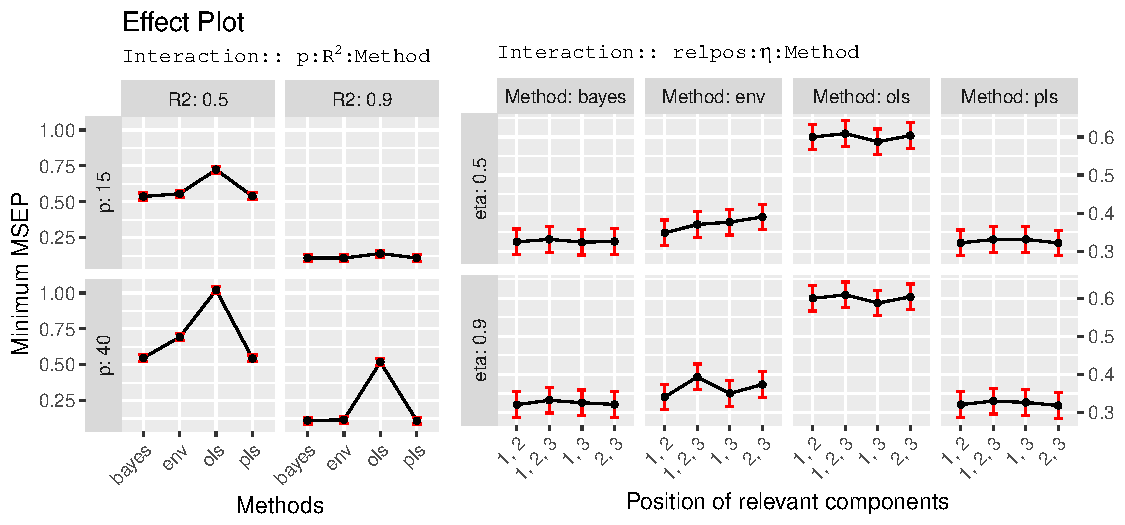
\includegraphics[width=\textwidth]{effect-plot}
\caption{Third order interaction effects}
\label{fig:effect-plot}
\end{figure}

The effect of the third order interaction between $p$, $\rho^2$ and {\tt Methods}, which we see in Figure~1~(left), shows that the maximum likelihood based estimation methods, in our case, the envelope and the ordinary least squares, perform poorly on data sets with large number of variables and low $\rho^2$. Still, the performance of the envelope is better than ordinary least squares also in situations where $p\sim n$. The interaction plots suggest that the Bayes PLS and ordinary PLS estimation methods are better and more stable on average than the two other methods.

Similarly, the effect of third order interaction between {\tt relpos}, $\eta$ and {\tt Method} in Figure~1~(right) shows that OLS method gives higher prediction error than other methods, but the effect of {\tt relpos} is small but notable for the envelope method. Again Bayes PLS and ordinary PLS are best.

The prediction error plots below are organized into four groups:
\begin{enumerate*}[label = \alph*)]
\item \label{lst:g1} $p = 15$, $\rho^2 = 0.5$;
\item \label{lst:g2} $p = 15$, $\rho^2 = 0.9$;
\item \label{lst:g3} $p = 40$, $\rho^2 = 0.5$ and
\item \label{lst:g4} $p = 40$, $\rho^2 = 0.9$.
\end{enumerate*}
The ordinary least squares prediction error is shown by a straight dotted line.

% \begin{center}
%   Figure-2 Here
% \end{center}

\begin{figure}[!ht]
\centering
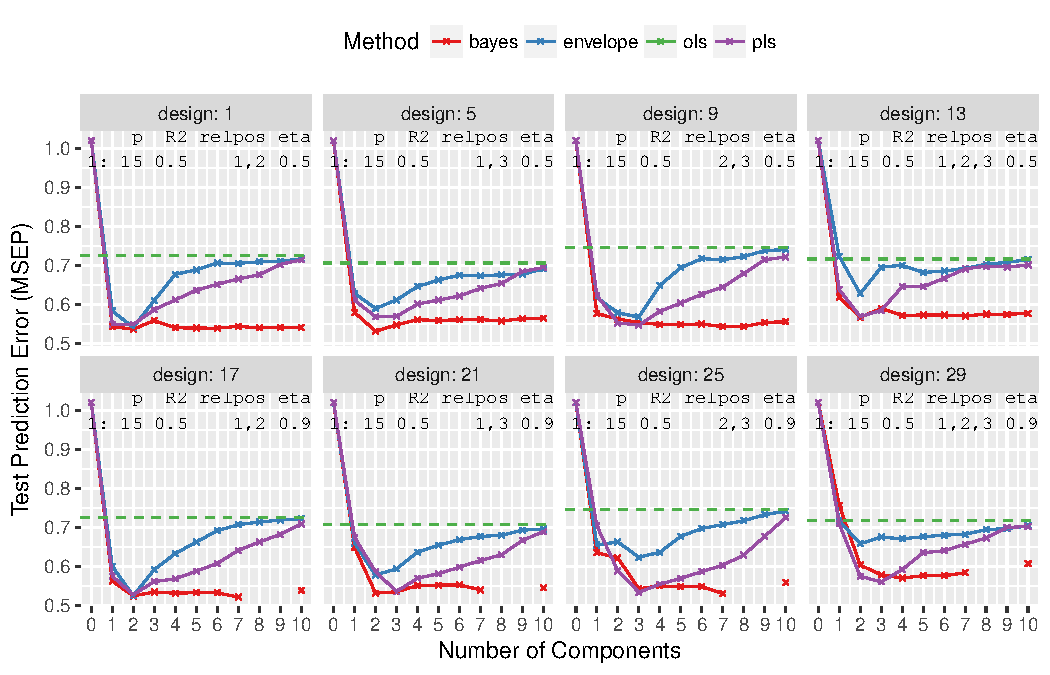
\includegraphics[width = \textwidth]{prediction-error-15-1.pdf}
\caption[Prediction Error - 1]{Average Prediction Error for designs with 15 predictor
variables where Coefficient of determination is 0.5}
\label{fig:pred-error-15-1}
\end{figure}

In group~\ref{lst:g1}, with small number of variables $(p \ll n)$ and noisy data
$(\rho^2 = 0.5)$, Figure~2 shows that all the estimation
methods performed better than ordinary least squares for all designs in this
group, Bayes PLS being best in nearly all cases. Some convergence problems with Bayes PLS when eigenvalues decrease rapidly
can be ignored since the minimum MSEP is already obtained from fewer components.

% \begin{center}
%   Figure-3 Here
% \end{center}

\begin{figure}[!ht]
\centering
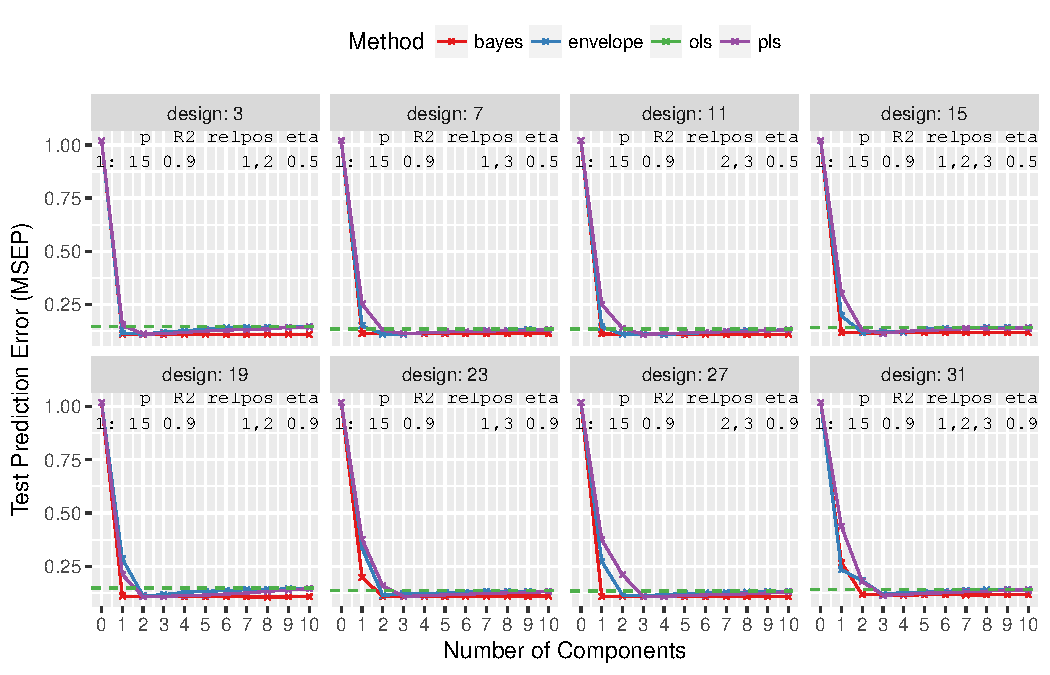
\includegraphics[width = \textwidth]{prediction-error-15-2.pdf}
\caption[Prediction Error - 2]{Average Prediction Error for designs with 15 predictor
variables where Coefficient of determination is 0.9}
\label{fig:pred-error-15-2}
\end{figure}

Having few variables rich with information $(\rho^2 = 0.9)$, the designs in group~\ref{lst:g2} (Figure~3) leads to easy prediction with low prediction error in general for all methods. All the methods including OLS have small MSEPs, but the other methods are still dominant. In most of the situations, Bayes PLS has reached minimum error with only one component. In this group, the performance of envelope is better than regular PLS and the minimum error for envelope is also achieved with fewer components.

% \begin{center}
%   Figure-4 Here
% \end{center}

\begin{figure}[!hptb]
\centering
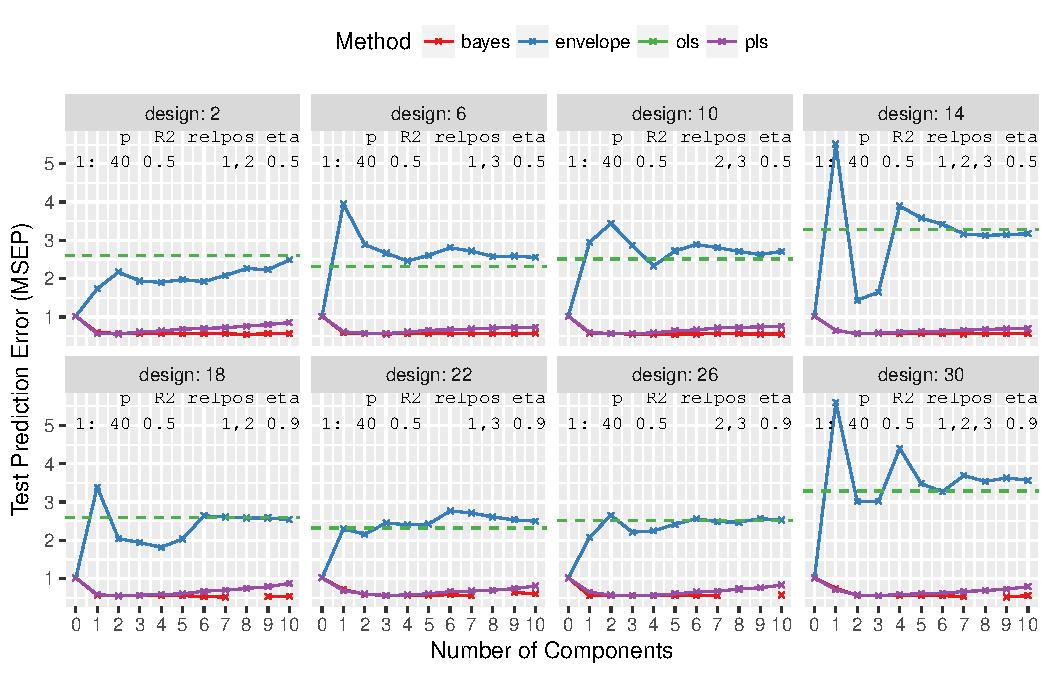
\includegraphics[width = 0.95\textwidth]{prediction-error-40-1.pdf}
\caption[Prediction Error - 3]{Average Prediction Error for designs with 40 predictor
variables where Coefficient of determination is 0.5}
\label{fig:pred-error-40-1}
\end{figure}

Low information content combined with many predictor variables characterize the designs in group~\ref{lst:g3} and prediction is in general difficult for these designs. In Figure~4, the methods based on maximum likelihood estimation performed poorly and often poorer than an average guess. Bayes PLS and regular PLS performed well, as in the previous designs.

% \begin{center}
%   Figure-5 Here
% \end{center}

\begin{figure}[!hptb]
\centering
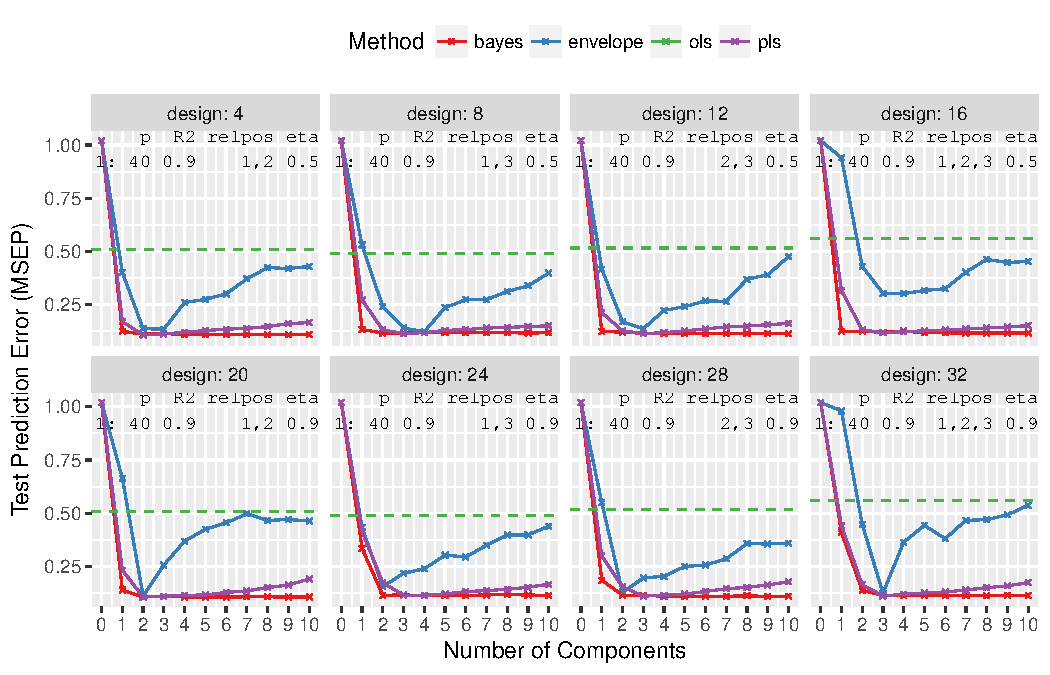
\includegraphics[width = 0.95\textwidth]{prediction-error-40-2.pdf}
\caption[Prediction Error - 4]{Average Prediction Error for designs with 40 predictor
variables where Coefficient of determination is 0.9}
\label{fig:pred-error-40-2}
\end{figure}

Although having 40 predictors $(p\sim n)$, all methods are performing well on the designs in group~\ref{lst:g4} due to rich information (high $\rho^2$). Figure~5 shows that in most of the situations (except in design-16), the envelope method has nearly attained true minimum error (0.1) and has outperformed OLS. However, its prediction error is still larger than Bayes PLS and PLS. Bayes PLS and PLS methods are highly stable and are closer to true minimum error. Both of these methods have outperformed OLS and the envelope methods. Further, Bayes PLS is able to obtain its minimum prediction error with only few components.

In general odinary PLS is very stable in all situations. It is extensible (lots of variants has been developed after its introduction), easy and less time consuming to fit than Bayes PLS and the envelope method. If the issue is to get closer prediction from squeezing information as much as possible, Bayes PLS will be an alternative. Its performance with fewer number of components is stable and better in all designs studied here. The envelope method performed better than OLS and the performance increased for informative data $(\rho^2 = 0.9)$. However, the increased error with additional component indicates low shrinkage effect of the
method.

Correlation between estimated and true regression coefficients $(\beta)$ along with the mean square error of estimation (MSE) is presented in Figure~6. In case of ordinary PLS and the envelope method, the correlation for design 1 from group~\ref{lst:g1} and design 3 from group~\ref{lst:g2}, both having 15 predictors, is high for small components. However for design 2 from group~\ref{lst:g3} and design 4 from group~\ref{lst:g4}, envelope methods exhibit sudden decrease in the correlation with corresponding increase in estimation error. The impressive prediction performance of Bayes PLS is also seen from the high correlation of estimated coefficients and true coefficients. In addition, the average MSE of regression for this methods is also small compared to others for all the components.

Although having low prediction error in case of envelope estimation method, the coefficient estimates are highly unstable for different components which we can see from its variation in correlation with true coefficients (Figure~6,~top. Bayes PLS and regular PLS estimates are more stable over different replicates and for different components (Figure~6, bottom) especially when $p\sim n$. This stability agrees with the low prediction error we have discussed before.

% \begin{center}
%  Figure-6 Here
% \end{center}

\begin{figure}[!ht]
  \centering
  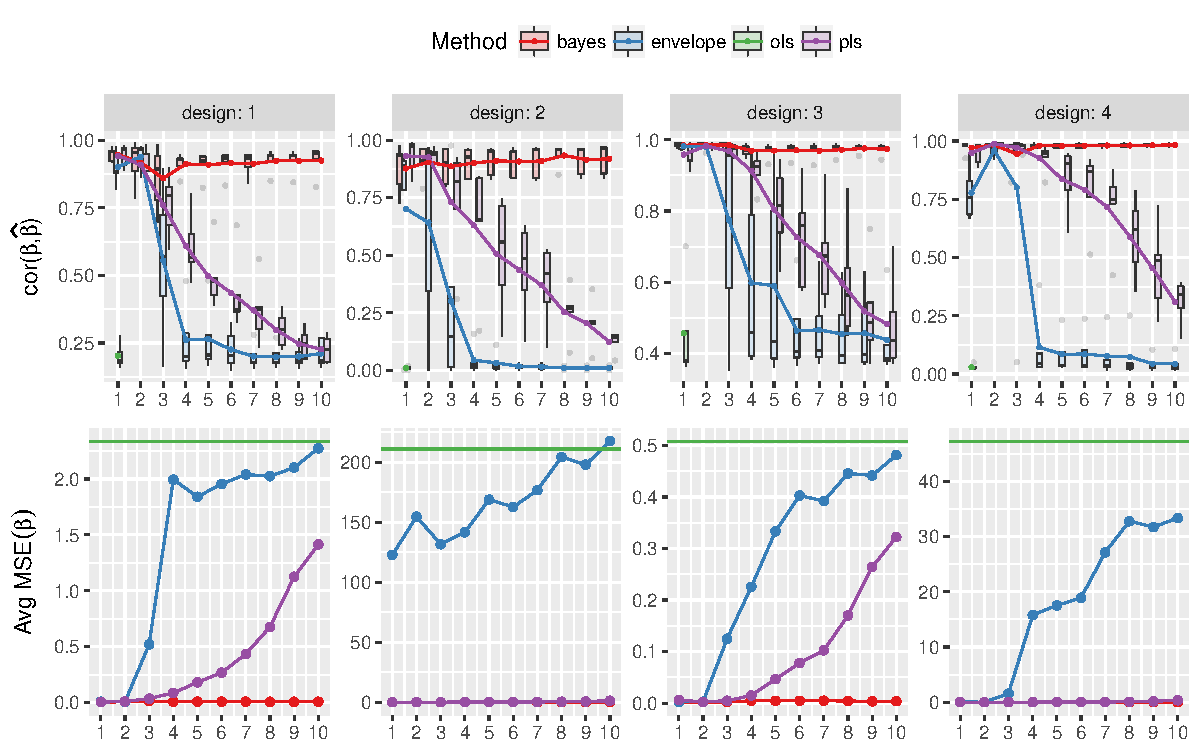
\includegraphics[width=\textwidth]{est-combined-plot.pdf}
  \caption{Correlation between true and estimated beta coefficient and Beta Estimation Error}
  \label{fig:est-error-combined}
\end{figure}

\section{Discussion}

The purpose of the present article has been to discuss the approach to PLS-regression via model reduction in the random $\bm{x}$ multiple regression model, and to compare estimators in this reduced model.

From simulations, the Bayes estimator under the PLS model seems to have very good properties. In virtually all of the 32 designs, the MSEP curve for Bayes PLS lie below that for ordinary PLS and also that for the maximum likelihood envelope model. A particularly desirable feature of Bayes-PLS is that the MSEP-curve seems to be almost flat for small values of $m$. Thus the error made by choosing a wrong number of components $m$ by crossvalidation must be expected to be small if $m$ is relatively small.

Envelope and Bayes PLS estimation methods, when compared with ordinary PLS methods, display better prediction performance (only when $p$ is small for the envelope method). However both of them have their disadvantages. The envelope method, as based on maximum likelihood, breaks down when $p$ approaches $n$, while Bayes PLS has time consuming computation, and in our simulations it failed to converge for some cases.

For practical purposes the ordinary PLS algorithm still seems to be a good option for prediction purposes, but from a statistical point of view, a closer study of its properties as $p\rightarrow\infty$ seems to be called for. We feel that the model approach of the present paper may give a good framework for such a study, both in terms of asymptotic expansions and in terms of further simulations. Such simulations may also include the cross-validated LASSO and other methods such as ridge regression, but note that these estimators ar derived from other considerations than that of predicting the effect of relevant components.

% Submissions are not required to reflect the precise reference formatting of the journal (use of italics, bold etc.), however it is important that all key elements of each reference are included.
\bibliography{references}

% \graphicalabstract{example-image-1x1}{Please check the journal's author guildines for whether a graphical abstract, key points, new findings, or other items are required for display in the Table of Contents.}

\end{document}
